\documentclass[12pt]{article}
\usepackage{algo,fullpage,url,amssymb,epsfig,color,xspace,tikz,amsmath}
\usepackage{graphicx}
\usepackage{float}
\usepackage[pdftitle={CS 486 Assignment 3},
pdfsubject={University of Waterloo, CS 486, Winter 2024},
pdfauthor={Arne Storjohann}]{hyperref}
\usepackage{algpseudocode,enumitem,calc,multicol}

\usepackage{listings}

\lstset{%
        language=python,
        keepspaces=true,
        basicstyle=\tiny\ttfamily,
       commentstyle=\tiny\itshape{},
       identifierstyle=\slshape{},
       keywordstyle=\bfseries,
       numbers=left,
       numberstyle=\tiny{},
       numberblanklines=false,
       inputencoding={utf8},
       columns=fullflexible,
       basewidth=.5em,
        fontadjust=true,
        tabsize=3,
        emptylines=*1,
       breaklines,
       breakindent=30pt,
        prebreak=\smash{\raisebox{-.5ex}{\hbox{\tiny$\hookleftarrow$}}},
    escapeinside={//*}{\^^M} % Allow to set labels and the like in comments starting with //*
	}


\renewcommand{\thesubsection}{Part \alph{subsection}}

\begin{document}

\begin{center}
  {\Large\bf University of Waterloo}\\ \vspace{3mm}
  {\Large\bf CS 486, Winter 2024}\\ \vspace{2mm}
  {\Large\bf Assignment 1}\\ \vspace{3mm}
\end{center}

\definecolor{care}{rgb}{0,0,0}
\def\question#1{\item[\bf #1.]}
\def\part#1{\item[\bf #1)]}
\newcommand{\pc}[1]{\mbox{\textbf{#1}}} % pseudocode

%%%%%%%%%%%%%%%%%%%%%%%%%%%%%%%%%%%%%%%%%%%%%
\subsection{} 
\begin{enumerate}
\part{1} Printout of the code:

\begin{lstlisting}
from math import log2
from queue import PriorityQueue
import matplotlib.pyplot as plt
import decimal

DEBUG = False

##### Variables ######
NUM_FEATURES = 0 # Define later
NUM_SAMPLE = 1500
ATHEISM_ID = 1
BOOKS_ID = 2
LABEL_STR = {ATHEISM_ID: "Atheism", BOOKS_ID: "Books" }

# We define P(x) as # belongs to atheism over total.

##### READING FILE ######

# Function to read label data, returning a dictionary mapping document ID to label
def read_label_data(file_name):
    label_data = {}
    with open(file_name, 'r') as file:
        lineNum = 0
        for line in file:
            lineNum += 1
            label_data[lineNum] = int(line.strip())
            # docId = line number
    file.close()
    return label_data

# Function to read word data, returning a dictionary mapping word ID to word
def read_word_data(file_name):
    word_data = {}
    with open(file_name, 'r') as file:
        lineNum = 0
        for line in file:
            lineNum += 1
            word_data[int(lineNum)] = line.strip()
            # wordId = line number
    # Define the Number of features
    global NUM_FEATURES
    NUM_FEATURES = lineNum
    file.close()
    return word_data

# Function to read train or test data
# document_data[n] = arrray of word_id that n+1'th doc have.
def read_document_data(file_name):
    document_data = {i: [] for i in range(1, NUM_SAMPLE + 1)} # 1 to 1500 
    with open(file_name, 'r') as file:
        for line in file:
            doc_id, word_id = line.strip().split()
            document_data[int(doc_id)].append(int(word_id))
    file.close()
    return document_data
    
##### TESTING ######

# 0.5 as we are ML
def predict_class(document, Theta_i_atheism, Theta_i_books, theta_atheism=0.5, theta_books=0.5):
    # Start with the theta_c
    prob_atheism = decimal.Decimal(theta_atheism)
    prob_books = decimal.Decimal(theta_books)
    
    # multiply all the likelihood
    for word_id in range(1, NUM_FEATURES + 1):
        if word_id in document:
            prob_atheism *= decimal.Decimal(Theta_i_atheism[word_id])
        else:
            prob_atheism *= decimal.Decimal(1 - Theta_i_atheism[word_id])
            
        if word_id in document:
            prob_books *= decimal.Decimal(Theta_i_books[word_id])
        else:
            prob_books *= decimal.Decimal(1 - Theta_i_books[word_id])
    
    normalized_prob_atheism = decimal.Decimal(prob_atheism / decimal.Decimal(prob_atheism + prob_books))
    # Return the class with the highest posterior probability
    if normalized_prob_atheism >= 0.5:
        return ATHEISM_ID
    else:
        return BOOKS_ID

##### MAIN ######

if __name__ == '__main__':
    
    # Reading data from files
    words = read_word_data('./dataset/words.txt')
    train_data = read_document_data('./dataset/trainData.txt')
    train_labels = read_label_data('./dataset/trainLabel.txt')
    test_data = read_document_data('./dataset/testData.txt')
    test_labels = read_label_data('./dataset/testLabel.txt')
    
    #### First calculate relative frequency of books belong to subreddit 'Atheism' or 'Books' ####
    total_count = 0
    atheism_count = 0
    books_count = 0

    for _, label in train_labels.items():
        total_count += 1
        if label == ATHEISM_ID:
            atheism_count += 1
        elif label == BOOKS_ID:
            books_count += 1
    
    theta_atheism = atheism_count / total_count
    theta_books = books_count / total_count
    
    if DEBUG:
        print(f"Total number of works: {NUM_FEATURES}")
        print(f"Total number of documents: {total_count}")
        print(f"Number of documents labeled as 'Atheism': {atheism_count}")
        print(f"Number of documents labeled as 'Books': {books_count}")
        print(f"Prior probability of 'Atheism' class: {theta_atheism:.4f}")
        print(f"Prior probability of 'Books' class: {theta_books:.4f}")
    
    #### Split train data for each label ####
    atheism_train_data = {}
    books_train_data = {}
    
    # Split the train_data based on the labels
    for doc_id, label in train_labels.items():
        if label == ATHEISM_ID:
            atheism_train_data[doc_id] = train_data[doc_id]
        elif label == BOOKS_ID:
            books_train_data[doc_id] = train_data[doc_id]
            
    #### calculate number of document (value) that have feature word_id (key) ####
    
    atheism_word_counts = {i: 0 for i in range(1, NUM_FEATURES + 1)} 
    for i in range(1, NUM_FEATURES + 1):
        # count the occurance of word_id = i
        for _, word_ids in atheism_train_data.items():
            if i in word_ids:
                atheism_word_counts[i] += 1

    books_word_counts = {i: 0 for i in range(1, NUM_FEATURES + 1)} 
    for i in range(1, NUM_FEATURES + 1):
        # count the occurance of word_id = i
        for _, word_ids in books_train_data.items():
            if i in word_ids:
                books_word_counts[i] += 1
                
    #### Account for Laplace correction when calculating the actual theta_i_1/0 ####
    
    Theta_i_atheism = {i: 0 for i in range(1, NUM_FEATURES + 1)}
    Theta_i_books = {i: 0 for i in range(1, NUM_FEATURES + 1)}
    
    for i in range(1, NUM_FEATURES + 1):
        Theta_i_atheism[i] = (atheism_word_counts[i] + 1) / (atheism_count + 2)
        Theta_i_books[i] = (books_word_counts[i] + 1) / (books_count + 2)
        
    ######################## PROCESSING FINISHED ########################
    
    print("")
        
    #### 10 most discriminative word features ####
    
    # Compute the log probabilities for each word
    log_prob_diffs = {}
    for word_id in range(1, NUM_FEATURES + 1):
        log_prob_atheism = log2(Theta_i_atheism[word_id])
        log_prob_books = log2(Theta_i_books[word_id])
        log_prob_diffs[word_id] = abs(log_prob_atheism - log_prob_books)

    # Sort the words by the most discriminative features
    most_discriminative = sorted(log_prob_diffs, key=log_prob_diffs.get, reverse=True)[:10]

    # Print the 10 most discriminative words
    print("10 Most Discriminative Word Features:")
    for word_id in most_discriminative:
        word = words[word_id]
        if DEBUG:
            print(f"Word: {word}, Difference in Log Probabilities: {log_prob_diffs[word_id]:.4f}")
        else:
            print(f"Word: {word}")
        
    print("")
    
    #### Predict the class for each document in the training set ####
    predicted_labels_train = {}
    for doc_id, document in train_data.items():
        predicted_labels_train[doc_id] = predict_class(document, Theta_i_atheism, Theta_i_books)

    # Calculate the accuracy
    correct_predictions_train = 0
    for doc_id, prediction in predicted_labels_train.items():
        if train_labels[doc_id] == prediction:
            correct_predictions_train += 1
            
    accuracy_train = correct_predictions_train / len(train_labels)

    print(f'Training accuracy of the Naive Bayes classifier (): {accuracy_train * 100:.2f}%')
    
    #### Predict the class for each document in the test set ####
    predicted_labels_test = {}
    for doc_id, document in test_data.items():
        predicted_labels_test[doc_id] = predict_class(document, Theta_i_atheism, Theta_i_books)

    # Calculate the accuracy
    correct_predictions_test = 0
    for doc_id, prediction in predicted_labels_test.items():
        if train_labels[doc_id] == prediction:
            correct_predictions_test += 1
            
    accuracy_test = correct_predictions_test / len(test_labels)

    print(f'Testing accuracy of the Naive Bayes classifier (): {accuracy_test * 100:.2f}%')
    
    print("")
    
\end{lstlisting}

\part{2} 10 most discriminative word features (from most to least, break ties randomly):

\texttt{christian, religion, atheism, books, christians, \\library, religious, libraries, novel, beliefs}

In my opinion, these words are indeed very good word features to classify the originated sub-reddit for each posts. All of these words are strongly associated to one of the topic "atheism" (like the words \texttt{christian}, \texttt{religion}, \texttt{atheism}, \texttt{christians}, \texttt{religious} and \texttt{beliefs}) or "books" (the words \texttt{books}, \texttt{library}, \texttt{libraries} and \texttt{novel}).

\part{3} 
\texttt{Training accuracy of the Naive Bayes classifier (): 90.27\%\\
Testing accuracy of the Naive Bayes classifier (): 74.47\%}

\part{4}
The naive Bayes model's assumption on the independency of words is not reasonable. Because for natural languages that we use, it has a structure with syntax and semantics where certain words are more likely to appear together.

For example, if a text has word \texttt{example}, then the likelihood of the word \texttt{for} appears in the same text is a lot higher, because \texttt{for example} is a popular phrase that people use.

Also, the meaning of a word can be context\-dependent in a lot cases. Words can have different meanings in different contexts and even the presence of certain words can influence the interpretation of other words.

These correlation between words means that the naive Bayes model's assumption on the words are not exactly reasonable, but it's a good simplification that works quite well in practice for certain applications such as spam detection and preliminary topic classification.

\part{5}
There are several things we can do to extend the Naive Bayes model to take into account of dependencies between words, they include but not limit to:

\begin{itemize}
	\item Extend the naive Bayes model into a more complex Bayesian Network that have edges between some word feature nodes will allow a word feature to be dependent to some other word features, which would allow the model to account for some dependencies between word features.
	
	\item Instead of use individual words as features with Naive Bayes model, we can instead use a sequence of few words ($n$-gram, note that our word features is where $n=1$) as features instead. This will allow the model to take into account some dependencies between words that often appear together.
	
\end{itemize}

\part{6}

If I were to use MAP learning instead of ML learning under the setting of continuous parameter $\theta$, then I will need to calculate the most likely posterior hypothesis $\theta ^* = \text{argmax}_\theta P(d | \theta)P(\theta)$, where $P(\theta)$ is the prior of the hypothesis (every parameter has a prior), instead of what ML required, which is the hypothesis that makes the data most likely $\theta = \text{argmax}_\theta P(d | \theta)$ (where we assumed a uniform prior, similar as what I did in my function \texttt{predict\_class()}, so we just omitted it), then take derivative of the RHS making it equal 0. After this, we find the most likely posterior hypothesis $\theta$, then make prediction use this value along with Laplace correction in a similar manner.

\iffalse
For the code I will first need to define some prior probability for the parameters (probabilities of the presence of words given the document's sub-reddit), even though this might not be too much of a issue because our dataset is rather large and the model will eventually forget the prior.

Then, instead of calculating the probability directly on two classification hypothesis under parameters (likelihood $\theta$ by dividing number of document have a certain word feature by total number of document under one sub-reddit) we previously calculated from train data and pick the larger one as our prediction, I will need to calculate these parameters with the inclusion of prior distribution (like add values to the numerator and denominator). Also when predicting, we will need to adjust the prior probability of the class if they are known and not uniform. Which is assumed to be uniform by my default parameter to function \texttt{predict\_class()}.
\fi
\end{enumerate}


%%%%%%%%%%%%%%%%%%%%%%%%%%%%%%%%%%%%%%%%%%%%%
%%%%%%%%%%%%%%%%%%%%%%%%%%%%%%%%%%%%%%%%%%%%%
\newpage
\subsection{}
The content of Q1 is submit to marmoset. 
\begin{enumerate}
\part{1} 
Code for k-fold cross validation with $k=5$:

\begin{lstlisting}
import numpy as np
import pandas as pd
import matplotlib.pyplot as plt

from neural_net import NeuralNetwork
from operations import *

from sklearn.model_selection import KFold

def load_dataset(csv_path, target_feature):
    dataset = pd.read_csv(csv_path)
    t = np.expand_dims(dataset[target_feature].to_numpy().astype(float), axis=1)
    X = dataset.drop([target_feature], axis=1).to_numpy()
    return X, t

X, y = load_dataset("data/wine_quality.csv", "quality")

n_features = X.shape[1]

# Hyperparameters and settings
n_splits = 5
epochs = 500
learning_rate = 0.001

# Initialize k-fold cross-validation
kf = KFold(n_splits=n_splits, shuffle=True, random_state=None)

# Initialize variables to store metrics
fold_losses = []
fold_maes = []
epoch_losses = np.zeros((n_splits, epochs))

# neural network architecture
layer_sizes = [32,32,16,1]
activations = [ReLU(), ReLU(), Sigmoid(), Identity()]


# K-Fold Cross Validation
for fold, (train_idx, val_idx) in enumerate(kf.split(X)):
    print(f"Training on fold {fold+1}/{n_splits}...")
    
    # Split data into training and validation sets
    X_train, X_val = X[train_idx], X[val_idx]
    y_train, y_val = y[train_idx], y[val_idx]
    
    # Initialize the neural network
    nn = NeuralNetwork(n_features=n_features, 
                       layer_sizes=layer_sizes, 
                       activations=activations, 
                       loss=MeanSquaredError(), 
                       learning_rate=learning_rate)
    
    # Train the neural network
    W, epoch_loss = nn.train(X_train, y_train, epochs=epochs)
    epoch_losses[fold, :] = epoch_loss
    
    # Evaluate on validation set
    mae = nn.evaluate(X_val, y_val, mean_absolute_error)
    fold_maes.append(mae)
    print(f"Fold {fold+1} MAE: {mae}")

# Average training loss over folds for each epoch
average_epoch_losses = epoch_losses.mean(axis=0)
std_deviation_maes = np.std(fold_maes)
average_mae = np.mean(fold_maes)

# Output the results
print(f"Average MAE over all folds: {average_mae}")
print(f"Standard Deviation of MAE over all folds: {std_deviation_maes}")

# Plot the results
plt.plot(range(epochs), average_epoch_losses, label='Average Training Loss')
plt.xlabel('Epoch')
plt.ylabel('Average Loss')
plt.title('Training Loss Over Epochs')
plt.legend()
plt.show()

\end{lstlisting}

\newpage
\part{2} 
Size of layers: \texttt{[32,32,16,1]} \\
Layer used in my neural network: \texttt{[ReLU(), ReLU(), Sigmoid(), Identity()]}\\
(Same as the one given in \texttt{neural\_net.py})\\

\part{3}
Plot:\\
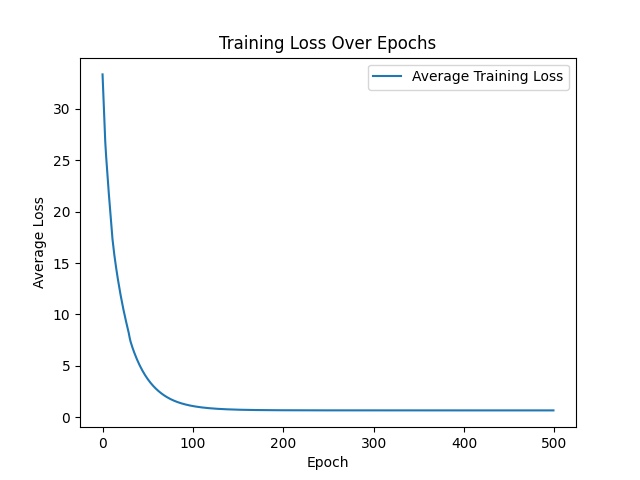
\includegraphics[width=\textwidth /3 * 2]{Q2/Q2.png}\\

\part{4}
\texttt{Average MAE over all folds: 0.6851463920029073\\
Standard Deviation of MAE over all folds: 0.01271361092488064}

\end{enumerate}

%%%%%%%%%%%%%%%%%%%%%%%%%%%%%%%%%%%%%%%%%%%%%
%%%%%%%%%%%%%%%%%%%%%%%%%%%%%%%%%%%%%%%%%%%%%

\end{document}
